\section{Appendices}
% NOTE NAMING OF FIGURES IN APPENDIX! APPENDIX X: asdfasdf

\subsection{PAAVO 2019 postal code areas}
\justify

% Longtable allows tables to span multiple pages. Not possible with tabularx
\begin{center}
    \begin{longtable}{|l l l l|} 
        \hline
        Postal code & Name (fi) & Name (sv) & Municipality \\ [0.5ex]
        \hline\hline
        \endhead % all lines above this will be repeated on every page
        00100 & Helsinki Keskusta - Etu-Töölö & Helsingfors centrum - Främre Tölö & 091 \\ [0.5 ex] \hline
        00120 & Punavuori & Rödbergen & 091 \\ [0.25ex] \hline
        00130 & Kaartinkaupunki & Gardesstaden & 091 \\ [0.25ex] \hline
        00140 & Kaivopuisto - Ullanlinna & Brunnsparken - Ulrikasborg & 091 \\ [0.25ex] \hline
        00150 & Eira - Hernesaari & Eira - Ärtholmen & 091 \\ [0.25ex] \hline
        00160 & Katajanokka & Skatudden & 091 \\ [0.25ex] \hline
        00170 & Kruununhaka & Kronohagen & 091 \\ [0.25ex] \hline
        00180 & Kamppi - Ruoholahti & Kampen - Gräsviken & 091  \\ [0.25ex] \hline
        00190 & Suomenlinna & Sveaborg & 091 \\ [0.25ex] \hline
        00200 & Lauttasaari & Drumsö & 091 \\ [0.25ex] \hline
        00210 & Vattuniemi & Hallonnäs & 091 \\ [0.25ex] \hline
        00220 & Jätkäsaari & Busholmen & 091 \\ [0.25ex] \hline
        00230 & Ilmala & Ilmala & 091 \\ [0.25ex] \hline
        00240 & Länsi-Pasila & Västra Böle & 091 \\ [0.25ex] \hline
        00250 & Taka-Töölö & Bortre Tölö & 091 \\ [0.25ex] \hline
        00260 & Keski-Töölö & Mellersta Tölö & 091 \\ [0.25ex] \hline
        00270 & Pohjois-Meilahti & Norra Mejlans & 091 \\ [0.25ex] \hline
        00280 & Ruskeasuo & Brunakärr & 091 \\ [0.25ex] \hline
        00290 & Meilahden sairaala-alue & Mejlans sjukhusområde & 091 \\ [0.25ex] \hline
        00300 & Pikku Huopalahti & Lillhoplax & 091 \\ [0.25ex] \hline
        00310 & Kivihaka & Stenhagen & 091 \\ [0.25ex] \hline
        00320 & Etelä-Haaga & Södra Haga & 091 \\ [0.25ex] \hline
        00330 & Munkkiniemi & Munksnäs & 091 \\ [0.25ex] \hline
        00340 & Kuusisaari-Lehtisaari & Granö-Lövö & 091 \\ [0.25ex] \hline
        00350 & Munkkivuori-Niemenmäki & Munkshöjden-Näshöjden & 091\\ [0.25ex] \hline
        00360 & Pajamäki & Smedjebacka & 091 \\ [0.25ex] \hline
        00370 & Reimarla & Reimars & 091 \\ [0.25ex] \hline
        00380 & Pitäjänmäen teollisuusalue & Sockenbacka industriområde & 091 \\ [0.25ex] \hline
        00390 & Konala & Kånala & 091 \\ [0.25ex] \hline
        00400 & Pohjois-Haaga & Norra Haga & 091 \\ [0.25ex] \hline
        00410 & Malminkartano & Malmgård & 091 \\ [0.25ex] \hline
        00420 & Kannelmäki & Gamlas & 091 \\ [0.25ex] \hline
        00430 & Maununneva & Magnuskärr & 091 \\ [0.25ex] \hline
        00440 & Lassila & Lassas & 091 \\ [0.25ex] \hline
        00500 & Sörnäinen & Sörnäs & 091 \\ [0.25ex] \hline
        00510 & Etu-Vallila - Alppila & Främre Vallgård - Alphyddan & 091 \\ [0.25ex] \hline
        00520 & Itä-Pasila & Östra Böle & 091 \\ [0.25ex] \hline
        00530 & Kallio & Berghäll & 091 \\ [0.25ex] \hline
        00540 & Kalasatama & Fiskhamnen & 091 \\ [0.25ex] \hline
        00550 & Vallila & Vallgård & 091 \\ [0.25ex] \hline
        00560 & Toukola-Vanhakaupunki & Majstad-Gammelstad & 091 \\ [0.25ex] \hline
        00570 & Kulosaari & Brändö & 091 \\ [0.25ex] \hline
        00580 & Verkkosaari & Nätholmen & 091 \\ [0.25ex] \hline
        00590 & Kaitalahti & Hålvik & 091 \\ [0.25ex] \hline
        00600 & Koskela-Helsinki & Forsby-Helsingfors & 091 \\ [0.25ex] \hline
        00610 & Käpylä & Kottby & 091 \\ [0.25ex] \hline
        00620 & Metsälä-Etelä-Oulunkylä & Krämertsskog-Södra Åggelby & 091 \\ [0.25ex] \hline
        00630 & Maunula-Suursuo & Månsas-Storkärr & 091 \\ [0.25ex] \hline
        00640 & Oulunkylä-Patola & Åggelby-Dammen & 091 \\ [0.25ex] \hline
        00650 & Veräjämäki & Grindbacka & 091 \\ [0.25ex] \hline
        00660 & Länsi-Pakila & Västra Baggböle & 091 \\ [0.25ex] \hline
        00670 & Paloheinä & Svedängen & 091 \\ [0.25ex] \hline
        00680 & Itä-Pakila & Östra Baggböle & 091 \\ [0.25ex] \hline
        00690 & Tuomarinkylä-Torpparinmäki & Domarby-Torparbacken & 091 \\ [0.25ex] \hline
        00700 & Malmi & Malm & 091 \\ [0.25ex] \hline
        00710 & Pihlajamäki & Rönnbacka & 091 \\ [0.25ex] \hline
        00720 & Pukinmäki-Savela & Bocksbacka-Lerstrand & 091 \\ [0.25ex] \hline
        00730 & Tapanila & Mosabacka & 091 \\ [0.25ex] \hline
        00740 & Siltamäki & Brobacka & 091 \\ [0.25ex] \hline
        00750 & Puistola & Parkstad & 091 \\ [0.25ex] \hline
        00760 & Suurmetsä & Storskog & 091 \\ [0.25ex] \hline
        00770 & Jakomäki - Alppikylä & Jakobacka - Alpbyn & 091 \\ [0.25ex] \hline
        00780 & Tapaninvainio & Staffansslätten & 091 \\ [0.25ex] \hline
        00790 & Viikki & Vik & 091 \\ [0.25ex] \hline
        00800 & Länsi-Herttoniemi & Västra Hertonäs & 091 \\ [0.25ex] \hline
        00810 & Herttoniemi & Hertonäs & 091 \\ [0.25ex] \hline
        00820 & Roihuvuori & Kasberget & 091 \\ [0.25ex] \hline
        00830 & Tammisalo & Tammelund & 091 \\ [0.25ex] \hline
        00840 & Laajasalo & Degerö & 091 \\ [0.25ex] \hline
        00850 & Jollas & Jollas & 091 \\ [0.25ex] \hline
        00860 & Santahamina & Sandhamn & 091 \\ [0.25ex] \hline
        00870 & Etelä-Laajasalo & Södra Degerö & 091 \\ [0.25ex] \hline
        00880 & Roihupellon teollisuusalue & Kasåkerns industriområde & 091 \\ [0.25ex] \hline
        00890 & Itäsalmi & Östersundom & 091 \\ [0.25ex] \hline
        00900 & Puotinharju & Botbyhöjden & 091 \\ [0.25ex] \hline
        00910 & Puotila & Botby gård & 091 \\ [0.25ex] \hline
        00920 & Myllypuro & Kvarnbäcken & 091 \\ [0.25ex] \hline
        00930 & Itäkeskus-Marjaniemi & Östra centrum-Marudd & 091 \\ [0.25ex] \hline
        00940 & Kontula - Vesala & Gårdsbacka - Ärvings & 091 \\ [0.25ex] \hline
        00950 & Vartioharju & Botbyåsen & 091 \\ [0.25ex] \hline
        00960 & Pohjois-Vuosaari & Norra  Nordsjö & 091 \\ [0.25ex] \hline
        00970 & Mellunmäki & Mellungsbacka & 091 \\ [0.25ex] \hline
        00980 & Etelä-Vuosaari & Södra Nordsjö & 091 \\ [0.25ex] \hline
        00990 & Aurinkolahti & Solvik & 091 \\ [0.25ex] \hline
        01200 & Hakunila & Håkansböle & 092 \\ [0.25ex] \hline
        01230 & Vaarala & Fagersta & 092 \\ [0.25ex] \hline
        01260 & Itä-Hakkila & Östra Haxböle & 092 \\ [0.25ex] \hline
        01280 & Länsimäki & Västerkulla & 092 \\ [0.25ex] \hline
        01300 & Tikkurila & Dickursby & 092 \\ [0.25ex] \hline
        01340 & Leinelä & Lejle & 092 \\ [0.25ex] \hline
        01350 & Hiekkaharju & Sandkulla & 092 \\ [0.25ex] \hline
        01360 & Koivukylä-Havukoski & Björkby-Havukoski & 092 \\ [0.25ex] \hline
        01370 & Jokiniemi & Ånäs & 092 \\ [0.25ex] \hline
        01380 & Kuusikko-Hakkila & Sexan-Håkansböle & 092 \\ [0.25ex] \hline
        01390 & Ruskeasanta-Ilola & Rödsand-Gladas & 092 \\ [0.25ex] \hline
        01400 & Rekola & Räckhals & 092 \\ [0.25ex] \hline
        01420 & Päiväkumpu & Lövkulla & 092 \\ [0.25ex] \hline
        01450 & Korso & Korso & 092 \\ [0.25ex] \hline
        01480 & Mikkola & Mikkola & 092 \\ [0.25ex] \hline
        01510 & Kirkonkylä-Veromäki & Kyrkoby-Skattbacka & 092 \\ [0.25ex] \hline
        01520 & Tammisto & Rosendal & 092 \\ [0.25ex] \hline
        01530 & Veromiehenkylä & Skattmansby & 092 \\ [0.25ex] \hline
        01600 & Myyrmäki & Myrbacka & 092 \\ [0.25ex] \hline
        01610 & Kaivoksela & Gruvsta & 092 \\ [0.25ex] \hline
        01620 & Martinlaakso & Mårtensdal & 092 \\ [0.25ex] \hline
        01630 & Hämeenkylä & Tavastby & 092 \\ [0.25ex] \hline
        01640 & Hämevaara & Tavastberga & 092 \\ [0.25ex] \hline
        01650 & Vapaala & Friherrs & 092 \\ [0.25ex] \hline
        01660 & Varisto & Varistorna & 092 \\ [0.25ex] \hline
        01670 & Vantaanlaakso & Vandadalen & 092 \\ [0.25ex] \hline
        01680 & Askisto & Askis & 092 \\ [0.25ex] \hline
        01690 & Ylästö & Övitsböle & 092 \\ [0.25ex] \hline
        01700 & Kivistö & Kivistö & 092 \\ [0.25ex] \hline
        01710 & Pähkinärinne & Hasselbacken & 092 \\ [0.25ex] \hline
        01720 & Petikko & Petikko & 092 \\ [0.25ex] \hline
        01730 & Vantaanpuisto & Vandaparken & 092 \\ [0.25ex] \hline
        01740 & Tuupakan teollisuusalue & Stubbacka industriområde & 092 \\ [0.25ex] \hline
        01750 & Keimola & Käinby & 092 \\ [0.25ex] \hline
        01760 & Seutula & Sjöskog & 092 \\ [0.25ex] \hline
        01770 & Martinlaakson teollisuusalue & Mårtensdals industriområde & 092 \\ [0.25ex] \hline
        02100 & Tapiola & Hagalund & 049 \\ [0.25ex] \hline
        02110 & Otsolahti & Björnviken & 049 \\ [0.25ex] \hline
        02120 & Länsikorkee-Suvikumpu & Västerhöjden-Solhöjden & 049 \\ [0.25ex] \hline
        02130 & Pohjois-Tapiola & Norra Hagalund & 049 \\ [0.25ex] \hline
        02140 & Laajalahti & Bredvik & 049 \\ [0.25ex] \hline
        02150 & Otaniemi & Otnäs & 049 \\ [0.25ex] \hline
        02160 & Westend & Westend & 049 \\ [0.25ex] \hline
        02170 & Haukilahti & Gäddvik & 049 \\ [0.25ex] \hline
        02180 & Mankkaa & Mankans & 049 \\ [0.25ex] \hline
        02200 & Niittykumpu & Ängskulla & 049 \\ [0.25ex] \hline
        02210 & Olari & Olars & 049 \\ [0.25ex] \hline
        02230 & Matinkylä & Mattby & 049 \\ [0.25ex] \hline
        02240 & Friisilä & Frisans & 049 \\ [0.25ex] \hline
        02250 & Henttaa & Hemtans & 049 \\ [0.25ex] \hline
        02260 & Kaitaa & Kaitans & 049 \\ [0.25ex] \hline
        02270 & Finnoo-Eestinmalmi & Finno-Estmalmen & 049 \\ [0.25ex] \hline
        02280 & Malminmäki-Eestinlaakso & Malmbacka-Estdalen & 049 \\ [0.25ex] \hline
        02290 & Puolarmetsän sairaala & Bolarskogs sjukhus & 049 \\ [0.25ex] \hline
        02300 & Nöykkiönpuro & Nöykisbäcken & 049 \\ [0.25ex] \hline
        02320 & Espoonlahti & Esboviken & 049 \\ [0.25ex] \hline
        02330 & Saunalahti-Kattilalaakso & Bastvik-Kitteldalen & 049 \\ [0.25ex] \hline
        02340 & Latokaski & Ladusved & 049 \\ [0.25ex] \hline
        02360 & Soukka & Sökö & 049 \\ [0.25ex] \hline
        02380 & Suvisaaristo & Sommaröarna & 049 \\ [0.25ex] \hline
        02600 & Etelä-Leppävaara & Södra Alberga & 049 \\ [0.25ex] \hline
        02610 & Kilo & Kilo & 049 \\ [0.25ex] \hline
        02620 & Karakallio & Karabacka & 049 \\ [0.25ex] \hline
        02630 & Nihtisilta & Knektbro & 049 \\ [0.25ex] \hline
        02650 & Pohjois-Leppävaara & Norra Alberga & 049 \\ [0.25ex] \hline
        02660 & Lintuvaara & Fågelberga & 049 \\ [0.25ex] \hline
        02680 & Uusmäki & Nybacka & 049 \\ [0.25ex] \hline
        02700 & Kauniainen & Grankulla & 235 \\ [0.25ex] \hline
        02710 & Viherlaakso & Gröndal & 049 \\ [0.25ex] \hline
        02720 & Lähderanta & Källstrand & 049 \\ [0.25ex] \hline
        02730 & Jupperi & Jupper & 049 \\ [0.25ex] \hline
        02740 & Bemböle-Pakankylä & Bemböle-Backby & 049 \\ [0.25ex] \hline
        02750 & Sepänkylä-Kuurinniitty & Smedsby-Kurängen & 049 \\ [0.25ex] \hline
        02760 & Tuomarila-Suvela & Domsby-Södrik & 049 \\ [0.25ex] \hline
        02770 & Espoon Keskus & Esbo centrum & 049 \\ [0.25ex] \hline
        02780 & Kauklahti & Köklax & 049 \\ [0.25ex] \hline
        02810 & Gumböle-Karhusuo & Gumböle-Björnkärr & 049 \\ [0.25ex] \hline
        02820 & Nupuri-Nuuksio & Nupurböle-Noux & 049 \\ [0.25ex] \hline
        02860 & Siikajärvi & Siikajärvi & 049 \\ [0.25ex] \hline
        02920 & Niipperi & Nipert & 049 \\ [0.25ex] \hline
        02940 & Lippajärvi-Järvenperä & Klappträsk-Träskända & 049 \\ [0.25ex] \hline
        02970 & Kalajärvi & Kalajärvi & 049 \\ [0.25ex] \hline
        02980 & Lakisto & Lakisto & 049 \\ [1ex] \hline
        \caption{PAAVO postal code areas} \label{tab:recordstab2} % NB, not correct caption location
    \end{longtable}
\end{center}

\newgeometry{left=2cm, right=1cm, top=1.75cm, bottom=1.75cm}
\begin{sidewaysfigure}
    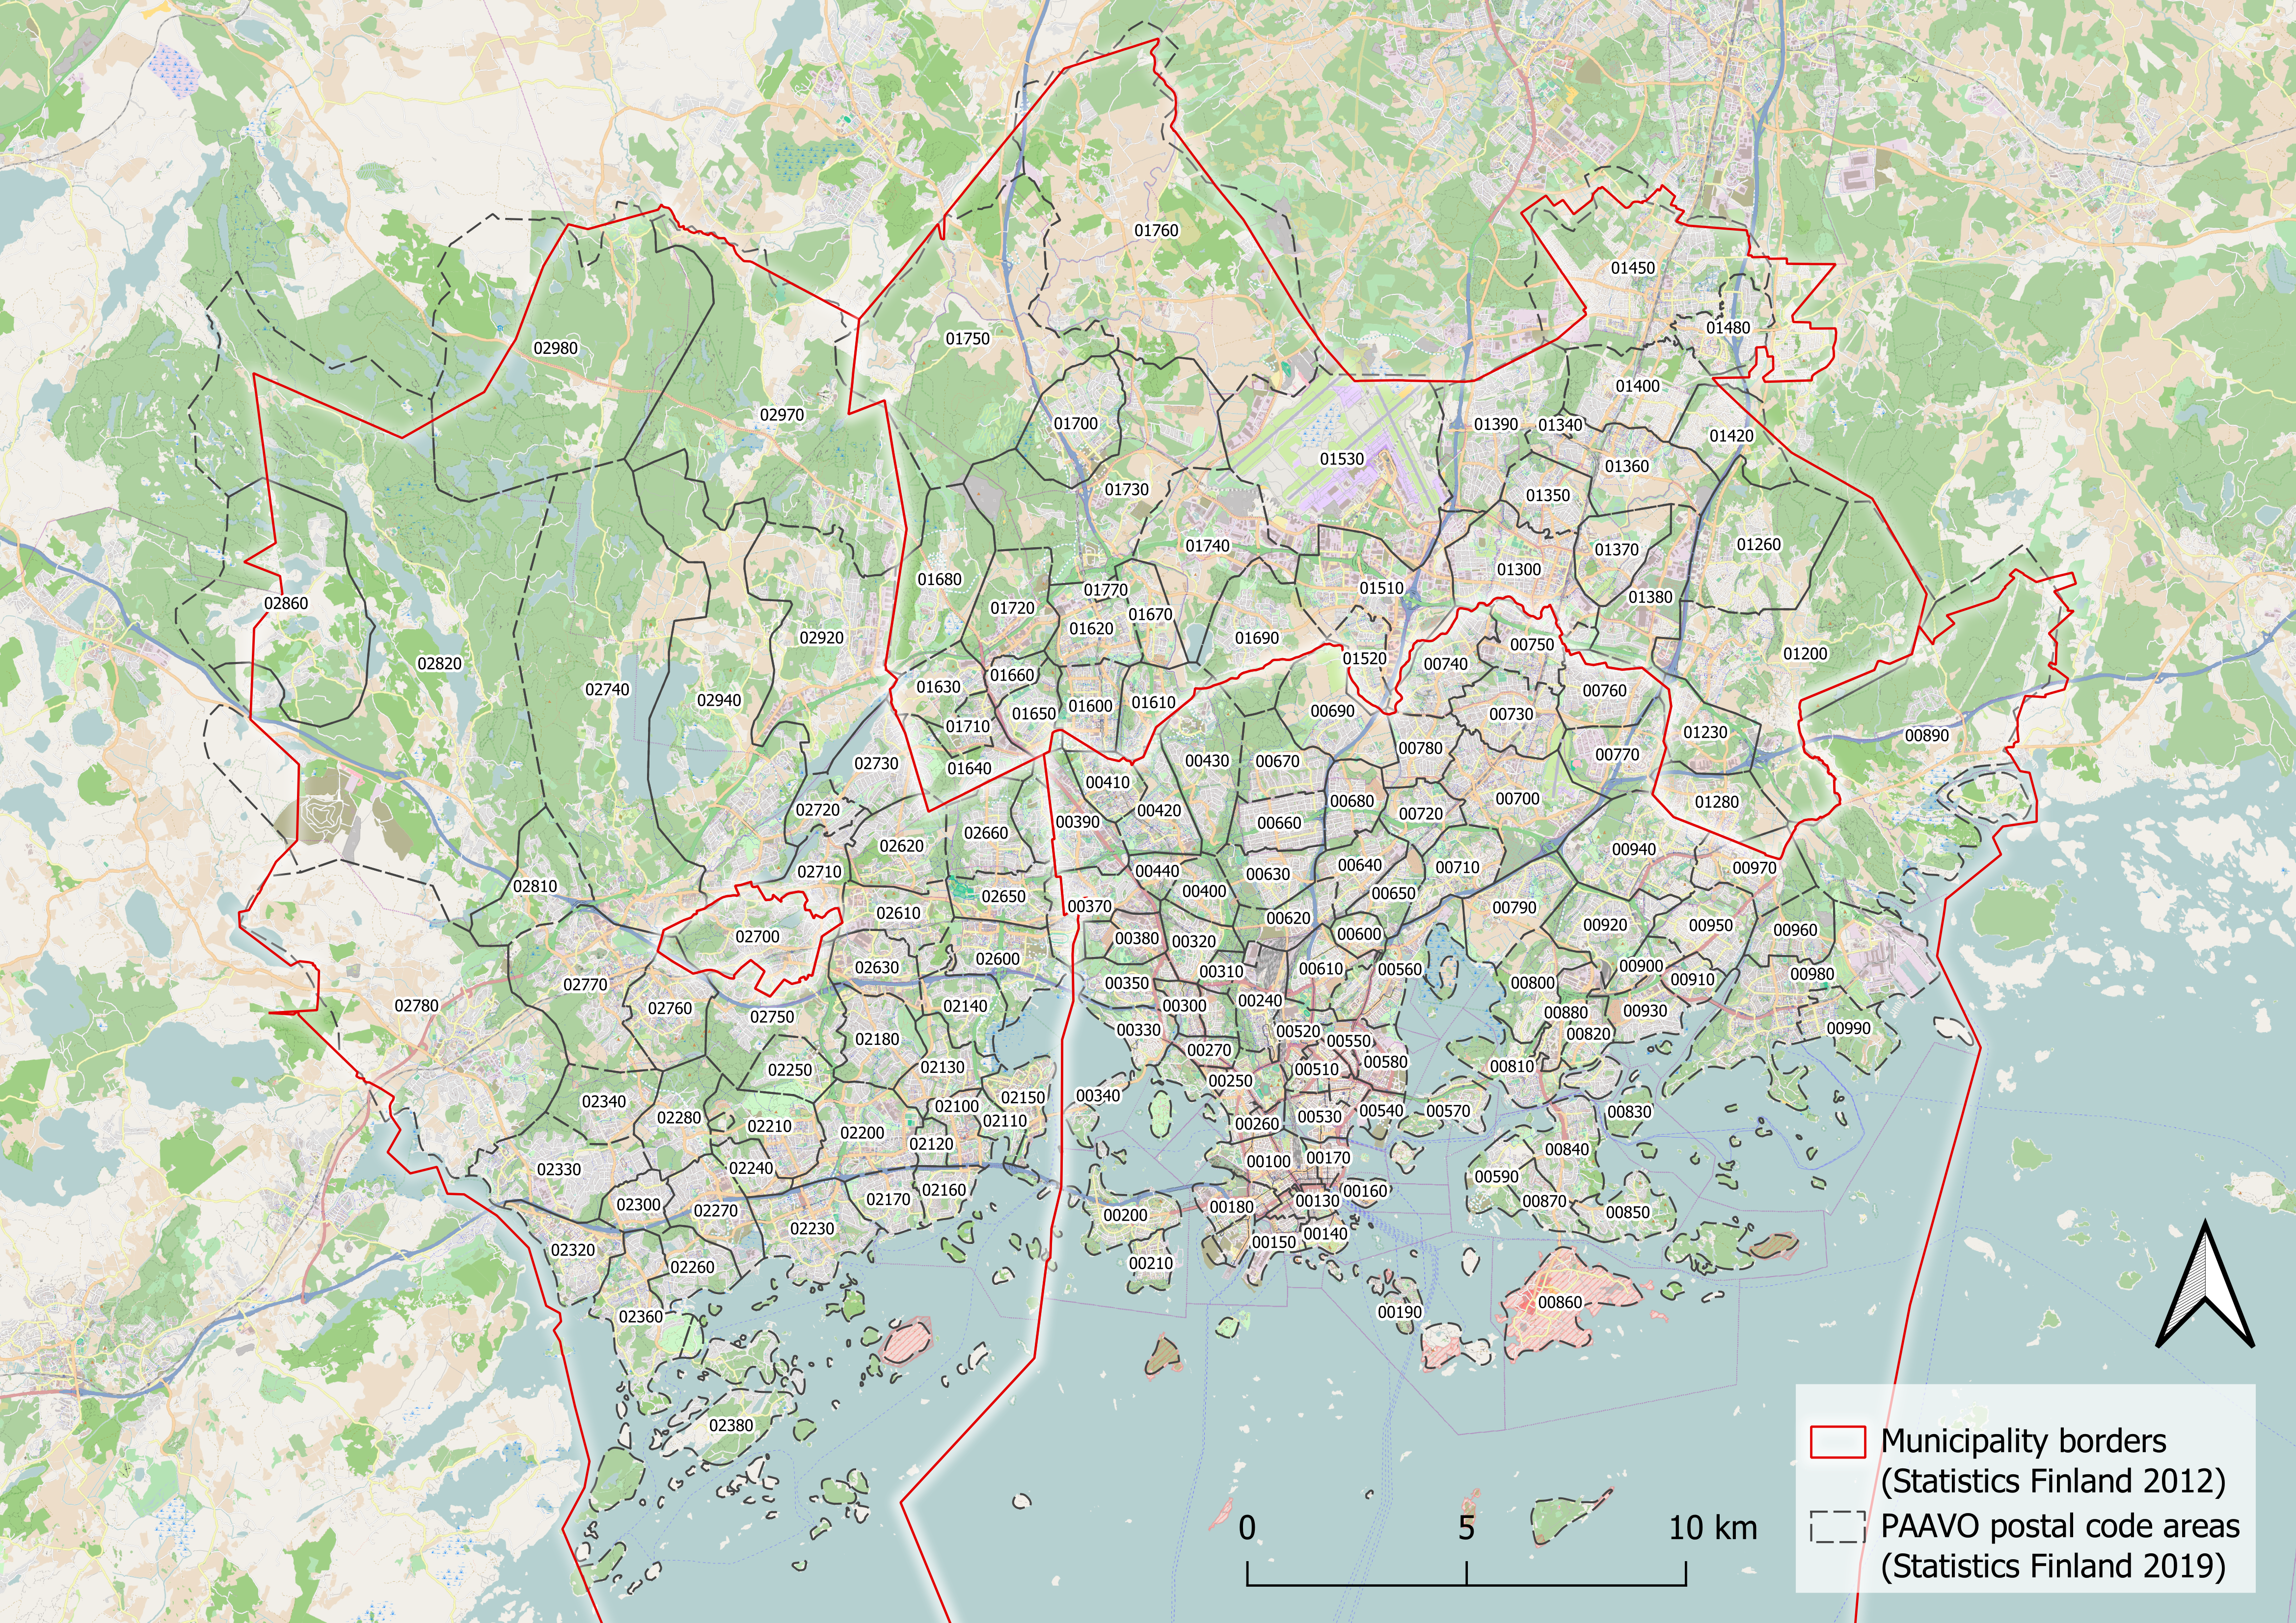
\includegraphics[width=\textwidth]{images/muns_postal_comparison.png}
    \caption{Comparison of municipality borders against PAAVO postal code areas.}
    \label{fig:muns_postal}
\end{sidewaysfigure}
\restoregeometry